\chapter{Securing \rustcore{}}
\label{sec:securercore}

%Continues from Code Migration (the redesign after the function-by-function
%rewrite), talk about \rustcore{} here.
%
%Rust has safe and unsafe code -> segregate unsafe code so that most of the
%hypervisor is written in safe Rust

\begin{figure}[ht]
\centering
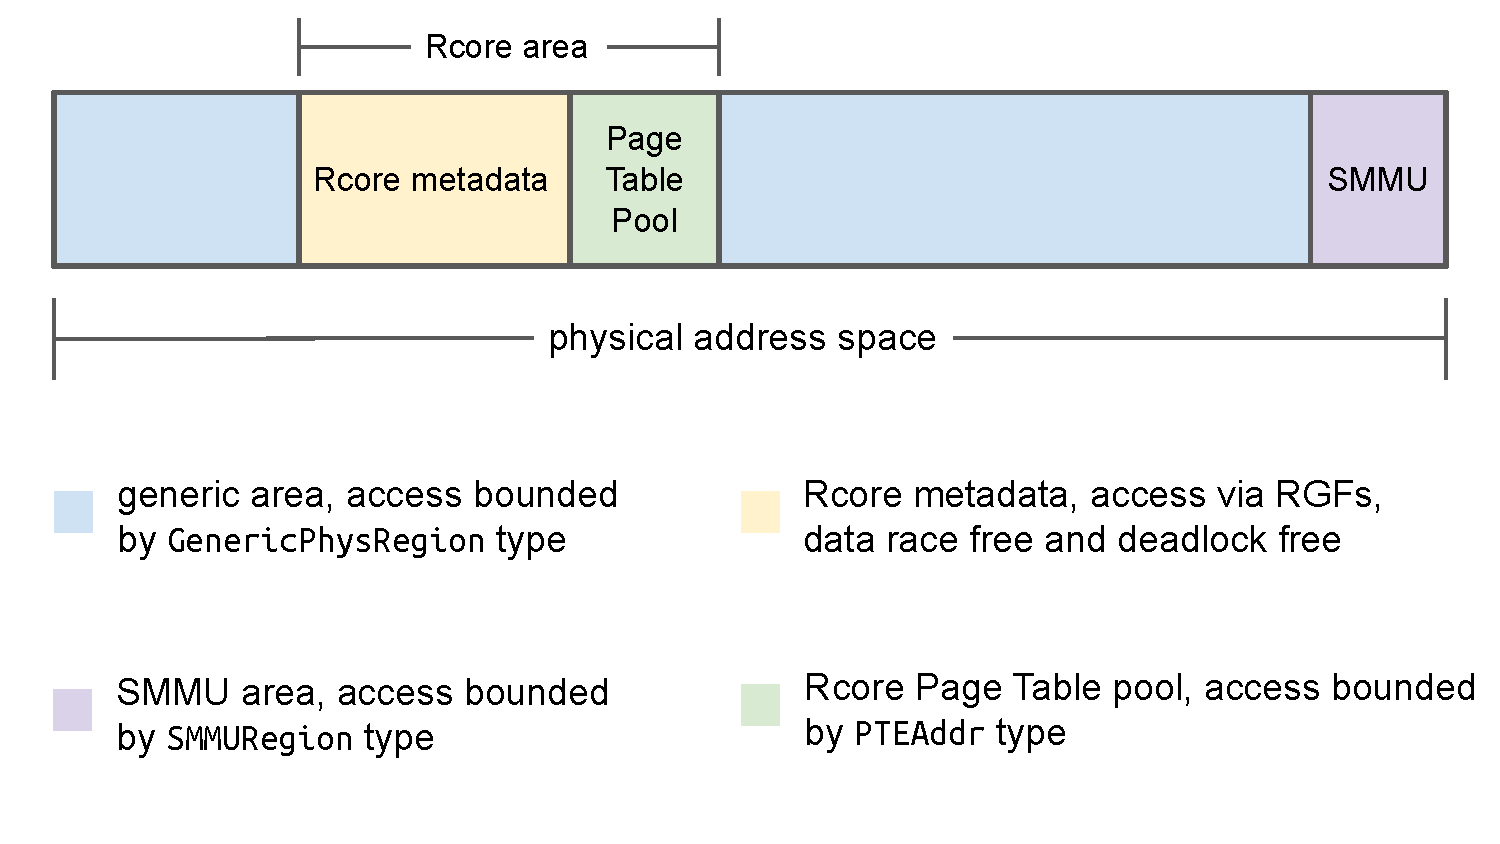
\includegraphics[width=1.00\textwidth]{figures/regions.pdf}
\caption{Memory Regions}
\label{fig:regions}
\end{figure}

\section{\rustcore{} Memory Regions}
\label{sec:rcoreregions}

\rustcore{}'s memory accesses are categorized into four disjoint regions:
\textit{\rustcore{} Metadata}, \textit{Page Table Pool},
\textit{SMMU Area}, and \textit{Generic Area}.
\rustcore{} metadata and \rustcore{} Page Table pool combined are referred to as
the \textit{\rustcore{} area} in the following.

\textbf{\rustcore{} Area.}
\rustcore{} needs a reserved memory region separated from the host Linux kernel
and all other VMs, named \textit{\rustcore{} area}, to provide its functionality.
The \rustcore{} area comprises the \rustcore{} Metadata and the \rustcore{} Page Table Pool.
The \rustcore{} Page Table Pool, as its name suggests, keeps private pools of physical pages
for NPTs and SMMU page tables so that \rustcore{} has complete control
over the permissions and the virtual-to-physical mappings of the memory
accessed by the host Linux kernel, VMs, and I/O devices. The \rustcore{} metadata,
on the other hand, is used for storing \rustcore{} metadata such as NPT information,
physical memory page ownership, VM states, SMMU page table metadata, etc.
We constructed custom types to store these \rustcore{} metadata.

\begin{table}
\begin{tabular}{ |p{0.2\linewidth}|p{0.7\linewidth}| }
\hline
\footnotesize \textbf{Name} & \footnotesize \textbf{Decription of Data} \\ \hline
\footnotesize vCPU context & \footnotesize The array that stores the state of each vCPU register. \\ \hline
\footnotesize VM info & \footnotesize The per-VM execution state metadata. \\ \hline
\footnotesize NPT info & \footnotesize The NPT pool allocation status. \\ \hline
\footnotesize PMEM info & \footnotesize The physical memory ownership and sharing status. \\ \hline
\footnotesize SMMU info & \footnotesize The SMMU management and page tables metadata. \\ \hline
\footnotesize SMMUPT info & \footnotesize The SMMU page table pool allocation status. \\ \hline
\end{tabular}
\vspace{0.2cm}
\caption{\rustcore{} metadata}
\label{tab:metadata}
\vspace{-0.4cm}
\end{table}

\textbf{SMMU Area.}
SMMU is accessed via MMIOs. \rustcore{} unmaps the SMMU
from the host NPT to trap-and-emulate its access to the SMMU. This
approach assures \rustcore{} has exclusive access to the SMMU.

\textbf{Generic Area.}
The \textit{Generic Area} refers to memory outside the \rustcore{} area and the SMMU area.
\rustcore{} needs to access this area to modify memory pages
belonging to the host or guests for VM services, such as zeroing a page
before transferring ownership from a guest back to the host during VM termination.

\section{Memory Region Isolation}

Raw pointer accesses are prohibited in safe Rust as they easily violate Rust’s
ownership model. As detailed in the upcoming paragraphs, we examine the need
for raw pointers for accessing the four regions described in \autoref{sec:rcoreregions}
and the measures are taken to guarantee their isolation,
even when employing unsafe Rust in their implementation.
We also deliberately made the
amount of unsafe code that contains raw pointer accesses small ($\sim$50 LOC).

\textbf{Raw Pointer Access: \rustcore{} Metadata.}
The RGFs return mutable references from a raw pointer, thus encapsulating the
raw pointer usages when the caller wishes to access \rustcore{} metadata
(\code{RcoreMetadata}).
All memory accesses done via RGFs are bounded in the range
from \code{RCORE\-\_\-META\-DATA\-\_\-PTR} to
\code{RCORE\-\_\-META\-DATA\-\_\-PTR + size\-of\-(Rcore\-Metadata)},
as accesses to non-array fields will not go out of bounds,
and Rust automatically adds runtime checks for the indices when array fields are accessed.
We manually check this range is only accessible by \rustcore{} and disjoint
from the page table pool and SMMU area by checking it is within the memory range unmapped from the
host Linux kernel for \rustcore{} and comparing the addresses with the page table pool area and SMMU area.
Hence, it is impossible for \rustcore{} metadata accesses to access
the other three regions accidentally.

\textbf{Raw Pointer Access: Generic Area.}
Generic area accesses are done by calculating raw addresses and writing to them
via raw pointers. Raw pointers are necessary here because system RAM is just a
range of flat address space to \rustcore{}. To ensure that code accessing the
generic area does not accidentally access the \rustcore{} area,
a new type called \code{GenericPhysRegion}
(\autoref{lst:genericphysslice}) has been created, which can only point to a
memory range in the generic area.
\code{GenericPhysRegion} only has one constructor, namely the \code{new}
method at line 2 in~\autoref{lst:genericphysslice}. This method verifies whether
the memory range specified by the arguments (start address \code{start\_addr} and
access size \code{size}) is contained within the bounds of the generic area.
If the specified range overlaps with the \rustcore{} area or the SMMU area, the constructor
returns a \code{None} variant, indicating that the construction has failed.
\autoref{lst:genericusage} shows an example usage of
\code{GenericPhysRegion}, which is a function that takes a physical frame number
(pfn), and clears the contents of the page.
The \code{GenericPhysRegion::new()} function is called at line 2 with the
physical address of the page (\code{pfn << PAGE\_SHIFT}) and its size
(\code{PAGE\_SIZE}) as arguments and returns a type of
\code{Option<GenericPhysRegion>}.
Next, we transform \code{Option} to \code{Result} type through \code{ok\_or}.
and use the \code{?} operator on the \code{Result} type to return the
contained value to \code{page} if it is an \code{Ok} variant.
Otherwise, \code{clear\_page} immediately returns \code{Err\-or}
without executing anything after line 2,
effectively propagating the absence of a value up the call stack.
The caller of \code{Generic\-Phys\-Region::\-new()} gets a
\code{GenericPhysRegion} if the check passes; otherwise,
\code{clear\_page} returns an \code{Error} type.
If successful, the page contents are cleared at line 4.

\begin{listing}[hbtp]
    \begin{minted}{rust}
impl GenericPhysRegion {
  pub fn new(start_addr: usize, size: usize) -> Option<Self> {
    let end = start_addr + size;
    // overlap check
    if (end > RCORE_AREA_START && RCORE_AREA_END > start_addr)
    || (end > SMMU_AREA_START && SMMU_AREA_END > start_addr) {
      return None;
    }
    Some(Self {
      start_addr,
      size,
    })
  }

  // returns a mutable `u8` slice for the caller
  // to access generic area memory
  pub fn as_slice(&self) -> &'static mut [u8] {
    // convert the physical address to the virtual address
    let va = pa_to_va(self.start_addr);
    unsafe {
      core::slice::from_raw_parts_mut(
        va as *mut u8, self.size,
      )
    }
  }
}
    \end{minted}
    \caption{\texttt{GenericPhysRegion} guarantees that every instance points to a valid generic area range}
    \label{lst:genericphysslice}
    \vspace{-0.2cm}
\end{listing}

\begin{listing}[hbtp]
    \begin{minted}{rust}
fn clear_page(pfn: usize) -> Result<()> {
  let page = GenericPhysRegion::new(pfn << PAGE_SHIFT, PAGE_SIZE).ok_or(Error::InvalidPfn)?;
  // the `fill` method for type &[u8] fills the slice with the value passed in
  page.as_slice().fill(0);
  Ok(())
}
    \end{minted}
    \caption{Example usage of \texttt{GenericPhysRegion}}
    \label{lst:genericusage}
    \vspace{-0.2cm}
\end{listing}

\textbf{Raw Pointer Access: Page Table Pool.}
\rustcore{} manages the host's and each VM's NPTs to control their access to
physical memory. SMMU page tables control I/O devices' memory access.
We also leveraged Rust's type system and created the
type \code{PTEAddr} (Page Table Entry Address). Each instance of type \code{PTEAddr}
points to an entry in the \rustcore{} Page Table Pool region.
Similar to \code{GenericPhysRegion}, \code{PTEAddr}'s constructor verifies whether the physical address provided as an
argument for the constructor is within the page table pool region in the \rustcore{}
area. If the address falls within the range, it is translated to the
corresponding virtual address and stored in a field of the
\code{PTEAddr} instance. Otherwise, the construction fails, and a
\code{None} is returned.
This type encapsulates the raw pointer address translation and bound
checks so for example the NPT walking code,
can guarantee it is accessing NPT entries in the
\rustcore{} page table pool area by using \code{PTEAddr}.

\textbf{Raw Pointer Access: SMMU.}
In a manner analogous to the generic area and page table pool, the type
\code{SMMURegion} for accessing SMMU is created.
\rustcore{} uses \code{SMMURegion} whenever it reads or writes SMMU registers.
\code{SMMURegion}'s \code{new} method takes the MMIO address and
verifies its inclusion within the SMMU region.
By consistently utilizing this type for SMMU accesses, SMMU accesses are
guaranteed to access the correct address region.
